%% ===========================================================================
%% ASP-DAC-style draft (IEEEtran conference format).
%% Self-contained: no internal-document references. Compile with pdflatex.
%%   pdflatex aspdac_ntt.tex  (x2 for references)
%% Figures are expected in ../figures/ (generated by scripts/plot_figures.py).
%% ===========================================================================
\documentclass[conference]{IEEEtran}

\usepackage{amsmath,amssymb}
\usepackage{amsthm}
\usepackage{graphicx}
\usepackage{booktabs}
\usepackage{array}
\usepackage{siunitx}
\usepackage{url}
\usepackage[hidelinks]{hyperref}
\graphicspath{{../figures/}}
\sisetup{group-separator={,},group-minimum-digits=4,detect-all}
\newtheorem{proposition}{Proposition}

\begin{document}

\title{A Measured Design-Space Exploration of Multivariate\\
Fermat-Modulus NTT on FPGA: Fixed-Width Compute\\
Scaling in Decomposition Depth}

\author{\IEEEauthorblockN{Anonymous Authors}
\IEEEauthorblockA{Affiliation\\
\texttt{email@domain}}}

\maketitle

\begin{abstract}
The Number-Theoretic Transform (NTT) over a Fermat-prime modulus
$q=2^{16}+1$ admits \emph{multiplier-less} (shift-only) butterflies, and a large
transform can be factored into a hierarchy of small sub-transforms through a
univariate-to-multivariate polynomial-ring map. While the underlying algorithm
is established, its hardware cost as a function of \emph{decomposition depth} has
not been systematically measured. This paper presents a fully placed-and-routed
design-space exploration of a multivariate Fermat-modulus NTT for negacyclic
polynomial multiplication on a Xilinx Alveo U280, sweeping the sub-transform
lane width $L\in\{4,8,16,32\}$ and the decomposition depth $d\in\{2,\dots,7\}$ ---
all thirteen configurations admissible under the Fermat-prime constraint
$N=L^{d}\le 32768$. Every configuration is functionally verified against a
reference model and synthesized to routed timing closure. Our central empirical
result is a \emph{fixed-width compute scaling} behavior: at a fixed lane width,
the compute fabric --- logic (LUT) and multipliers (DSP) --- stays essentially
flat as the depth $d$ --- and therefore the problem size $N=L^{d}$ --- grows,
while memory and latency grow with $N$. At $L=4$, the design uses exactly four
DSPs and $2.1$--$2.5$\,K LUTs across $d=3\ldots7$, a $256\times$ span in $N$
for only a $20\%$ increase in LUTs. This is enabled by a transpose-free
conflict-free memory organization whose interconnect width is $O(L)$ and is
therefore independent of both $d$ and $N$. We further report a candid comparison
against a state-of-the-art iterative Fermat-modulus NTT, which is more
area--time efficient at the small $N$ where both designs have published data; the
distinctive operating points of the hierarchical design are its minimal absolute
resource footprint and its validated operation across the entire Fermat-valid
depth range.
\end{abstract}

\begin{IEEEkeywords}
Number-theoretic transform, Fermat number transform, polynomial multiplication,
FPGA, design-space exploration, post-quantum cryptography.
\end{IEEEkeywords}

%% ===========================================================================
\section{Introduction}
%% ===========================================================================
Negacyclic polynomial multiplication in $\mathbb{Z}_q[x]/(x^{N}+1)$ is the
arithmetic kernel of lattice-based post-quantum cryptography and of fully
homomorphic encryption (FHE). The Number-Theoretic Transform (NTT) reduces the
$O(N^{2})$ schoolbook product to $O(N\log N)$ and is therefore the dominant
target for hardware acceleration~\cite{cooleytukey,longa2016}.

Two well-known algorithmic levers shape NTT hardware. First, choosing a
\emph{Fermat-prime} modulus $q=2^{k}+1$ makes the relevant roots of unity powers
of two, so that butterfly twiddle multiplications collapse to bit shifts; the
classical Fermat Number Transform (FNT)~\cite{agarwalburrus} exploits exactly
this, and it has recently been revisited for FHE
acceleration~\cite{kim2024fermat,xing2025}. Second, a large transform can be
\emph{factored} into a sequence of smaller sub-transforms with cross-twiddle
corrections, as in the four-step FFT~\cite{bailey1990} and its multi-step
generalizations on FPGA~\cite{kocer2024,wanggao2023}; this trades a single
all-to-all interconnect for several local passes and is the standard route to
large $N$ on bandwidth-limited devices.

Combining the two yields a \emph{multivariate Fermat NTT}: the polynomial ring is
re-expressed in $d$ variables, $N=L^{d}$, and each of the $d$ axes is transformed
by a shift-only $L$-point sub-NTT. The algorithm --- including the
univariate-to-multivariate ring map and the shift-only Fermat
property --- is established prior work~\cite{kim2024fermat,xing2025}. What is
\emph{not} established is a systematic, fully-measured answer to a concrete
hardware question: \emph{as the decomposition depth $d$ increases, how does the
implementation cost (logic, multipliers, memory, clock rate) actually scale?}
This question matters because depth is the knob that lets a fixed datapath reach
larger $N$, and the answer determines whether the approach genuinely keeps the
compute fabric fixed-width or merely shifts the cost into interconnect and memory.
Our conceptual hook is that, in this organization, \emph{decomposition depth
changes the schedule length but not the datapath width} --- a property we make
precise as an asymptotic characterization (Section~\ref{sec:asymp}) and confirm
on routed silicon.

\textbf{Contributions.} We make no claim to a new algorithm and no claim to beat
the state of the art on area--time efficiency. Our contributions are empirical
and architectural:
\begin{enumerate}
  \item A complete, placed-and-routed $L\times d$ design map (13 configurations,
  $N=64\ldots32768$) of a multivariate Fermat NTT on a single Alveo U280, each
  configuration functionally verified against a reference model
  (Section~\ref{sec:results}).
  \item An empirical \emph{fixed-width compute scaling} behavior and the
  architectural mechanism consistent with it: a transpose-free conflict-free
  memory organization with an $O(L)$ interconnect that does not grow with $d$ or
  $N$ (Sections~\ref{sec:arch},~\ref{sec:results}). The effect is strongest at
  narrow lane width; at large $L$ the absolute footprint is large.
  \item A candid comparison against a state-of-the-art iterative Fermat-modulus
  NTT, explicitly including the operating points where the hierarchical design
  loses (Section~\ref{sec:compare}).
\end{enumerate}
We state the boundary with prior art explicitly. \emph{Inherited:} the
multivariate Fermat-NTT algorithm (univariate-to-multivariate ring map, shift-only
butterflies)~\cite{kim2024fermat,xing2025}, and the idea of conflict-free banked
NTT memory~\cite{wanggao2023}. \emph{New here:} (i) the complete placed-and-routed
characterization across the \emph{entire} Fermat-valid depth range, where prior
work reports only shallow configurations; (ii) the asymptotic separation of
resource classes (Section~\ref{sec:asymp}) that identifies a width-invariant
compute regime --- a design objective orthogonal to the throughput optimization
of~\cite{xing2025}; and (iii) an exact, parameter-free cycle model validated
against all 13 measurements. We claim the \emph{characterization and the regime},
not the algorithm or the banking primitive in isolation.

\textbf{Scope.} Under $q=2^{16}+1$ the problem size is hard-capped at
$N\le 32768$ (Section~\ref{sec:bg}); we therefore characterize the entire
admissible grid rather than extrapolate beyond the modulus's reach.

%% ===========================================================================
\section{Background}\label{sec:bg}
%% ===========================================================================

\subsection{Negacyclic NTT}
To compute $c=a\cdot b \bmod (x^{N}+1)$ over $\mathbb{Z}_q$, let $\psi$ be a
primitive $2N$-th root of unity and $\omega=\psi^{2}$ a primitive $N$-th root.
The negacyclic product is obtained by a \emph{pre-twist} $\tilde a_i=a_i\psi^{i}$,
a length-$N$ cyclic NTT with root $\omega$, a point-wise product, an inverse NTT,
and a \emph{post-twist} by $\psi^{-i}$~\cite{longa2016}. The pre/post-twists and
the point-wise product require true modular multiplications; the NTT butterflies
do not, under the modulus below.

\subsection{Fermat modulus and the shift-only property}
We use $q=F_4=2^{16}+1=65537$. Because $\mathrm{ord}_q(2)=32$, an $S$-point NTT
has a root of unity that is a power of two if and only if $S\mid 32$; hence the
largest \emph{shift-only} sub-transform is $S_{\max}=32$. In a diminished-one
representation, multiplication by a power of two is a cyclic bit rotation, so an
$L$-point sub-NTT with $L\in\{4,8,16,32\}$ uses \emph{no} multipliers. The same
modulus imposes a hard ceiling: a primitive $2N$-th root exists only if
$2N\mid q-1=65536$, i.e.\ $N\le 32768$. Reaching larger $N$ requires either a
residue-number-system split into $\le\!32$K sub-products or a larger Fermat prime;
both are outside the scope of this study.

\subsection{Multivariate (multi-step) factorization}
Writing $N=L^{d}$ and indexing a coefficient by its mixed-radix digits
$i=\sum_{j=0}^{d-1} i_j L^{j}$, the length-$N$ transform factors into $d$ stages.
Stage $a$ applies an $L$-point NTT along axis $i_a$ (treating the data as a
$d$-dimensional $L\times\cdots\times L$ tensor), and adjacent stages are coupled
by cross-twiddle multiplications $\psi^{\,c}$ whose exponent $c$ is a product of
the transformed (frequency) digits and the axis index~\cite{bailey1990,
kim2024fermat}. This is the multidimensional Cooley--Tukey decomposition
specialized to equal radices; the univariate-to-multivariate ring map for the
negacyclic case is given in~\cite{kim2024fermat}.

%% ===========================================================================
\section{Architecture}\label{sec:arch}
%% ===========================================================================
Fig.~\ref{fig:arch} gives the top-level organization; the subsections detail the
shared datapath, the banking scheme, and the schedule.

\begin{figure}[t]
\centering
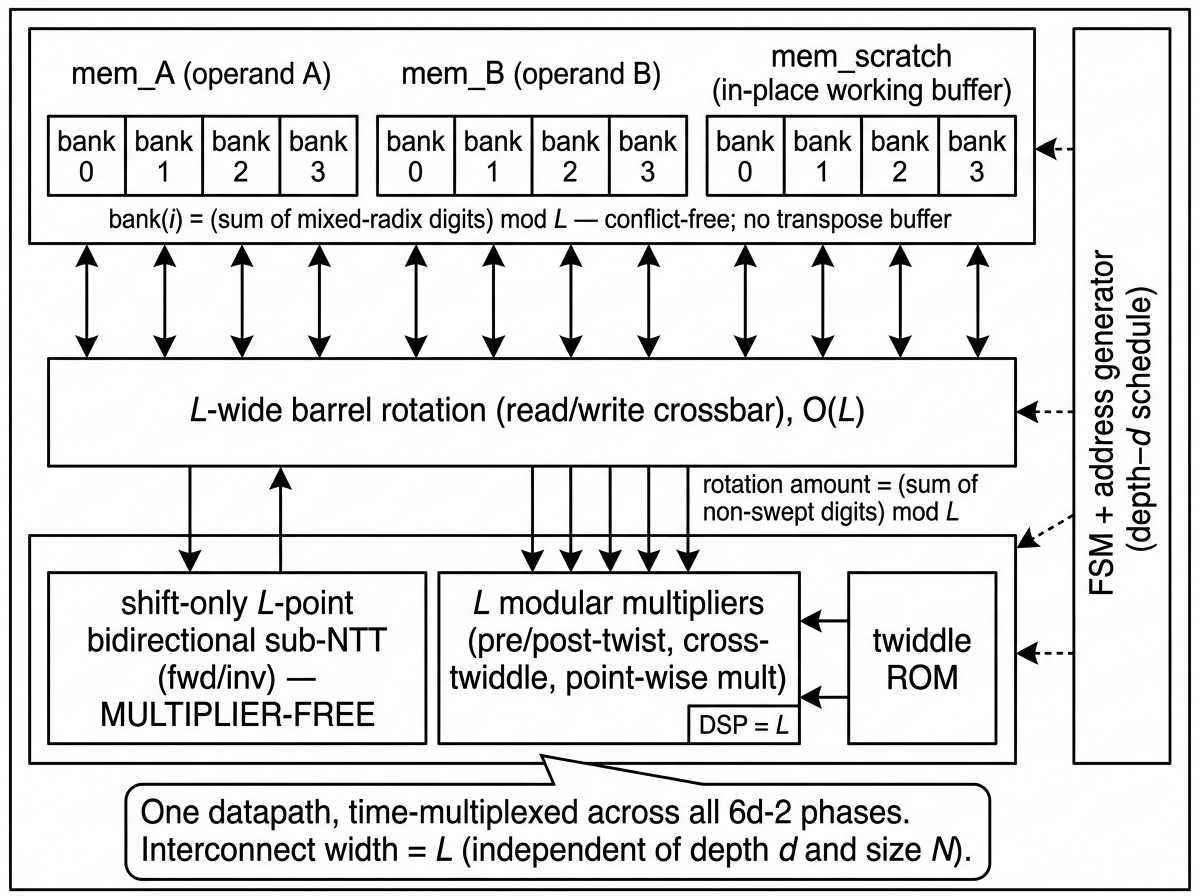
\includegraphics[width=\columnwidth]{fig1_architecture.png}
\caption{Shared-datapath architecture. Three banked memories (two operands, one
in-place scratch) connect through an $L$-wide barrel-rotation crossbar to a
single shift-only sub-NTT and an $L$-lane modular-multiplier array. The
conflict-free bank map makes every axis single-cycle accessible, so axis
switches are address remaps with no transpose buffer; the interconnect width is
$O(L)$, independent of $d$ and $N$.}
\label{fig:arch}
\end{figure}

\subsection{Shared $L$-lane datapath}
The design instantiates exactly one compute datapath, time-multiplexed across all
phases of a multiplication. It consists of (i) a single pipelined shift-only
$L$-point bidirectional sub-NTT, whose direction (forward/inverse) is selected
per issue, and (ii) an array of $L$ modular multipliers used by the pre-twist,
the $d-1$ cross-twiddle passes, the point-wise product, and the post-twist.
Because the sub-NTT is multiplier-free, the \emph{entire} design uses exactly
$L$ DSP blocks --- one per lane --- regardless of $d$ or $N$. A forward
transform of one operand costs $d$ sub-NTT passes and $d-1$ cross-twiddle passes;
a complete multiplication issues two forward transforms, one point-wise product,
and one inverse transform.

\subsection{Transpose-free conflict-free banking}
The classical hazard in multi-step NTT hardware is the inter-stage
\emph{corner-turn} (matrix transpose), which normally costs either a second
$N$-element ping-pong buffer or a dedicated transpose network. We avoid both with
a conflict-free bank assignment:
\begin{equation}
b(i)=\Big(\textstyle\sum_{j=0}^{d-1} i_j\Big)\bmod L,
\label{eq:bank}
\end{equation}
storing each coefficient in bank $b(i)$ at an intra-bank address formed from the
remaining digits.

\begin{proposition}\label{prop:cf}
For any axis $a\in\{0,\dots,d-1\}$, the $L$ coefficients of an $L$-point column
along axis $a$ --- i.e.\ indices agreeing in every digit except $i_a$ --- occupy
$L$ pairwise-distinct banks under~\eqref{eq:bank}.
\end{proposition}
\begin{proof}
Let $i,i'$ agree in every digit except axis $a$, with $i_a\neq i'_a$. By
\eqref{eq:bank}, $b(i)-b(i')\equiv i_a-i'_a \pmod L$. Since
$i_a,i'_a\in\{0,\dots,L-1\}$ and $i_a\neq i'_a$, we have $0<|i_a-i'_a|<L$, so the
difference is nonzero modulo $L$ and $b(i)\neq b(i')$. As the column contains
exactly the $L$ values $i_a=0,\dots,L-1$, their banks form a permutation of
$\{0,\dots,L-1\}$.
\end{proof}

Proposition~\ref{prop:cf} guarantees that an entire $L$-point column along any
axis is read or written in a single cycle with no bank conflict, for every
stage and every depth.
Crucially, switching the swept axis between stages changes only the
address-generation pattern; the data never moves. Consequently a multiplication
uses just three banked memories --- two to hold the operands (inherent to any
product) and one in-place working buffer --- with \emph{no} transpose buffer. The
only inter-bank wiring is an $L$-wide cyclic rotation (a barrel shifter) that
realigns lanes to banks, i.e.\ $O(L)$ multiplexing rather than the $O(L^{2})$ of a
full crossbar.

\subsection{Architectural asymptotics}\label{sec:asymp}
The design's resource classes scale along \emph{different} axes, and this
separation is the core of our characterization. Table~\ref{tab:asymp} states the
asymptotics; each row follows directly from the architecture above.

\begin{table}[t]
\centering
\caption{Asymptotic scaling of each resource class. Compute and interconnect
depend on the lane width $L$ only; size $N=L^{d}$ enters through memory and
runtime, not through the compute fabric.}
\label{tab:asymp}
\footnotesize
\begin{tabular}{lll}
\toprule
Resource class & Scaling & Reason\\
\midrule
Multipliers (DSP)      & $\Theta(L)$    & one mod-mult per lane\\
Sub-NTT / datapath LUT & $\Theta(L\log L)$ & one $L$-point shift-only kernel\\
Interconnect           & $\Theta(L)$    & $L$-wide barrel rotation (Prop.~1)\\
FSM / address logic    & $\Theta(d)$    & $6d-2$ phases, $d$-digit counters\\
On-chip memory         & $\Theta(N)$    & two operands $+$ one scratch\\
Latency (cycles)       & $\Theta(dN/L)$ & Eq.~\eqref{eq:cyc}\\
\bottomrule
\end{tabular}
\end{table}

The consequence is the paper's thesis: \emph{the compute fabric (DSP and
datapath LUT) and the interconnect are functions of $L$ alone and are
independent of the depth $d$ and the size $N=L^{d}$.} Increasing $d$ lengthens
the schedule ($\Theta(d)$ control, $\Theta(dN/L)$ cycles) and grows memory
($\Theta(N)$), but does not widen the datapath or the interconnect. This is a
different design objective from throughput-optimized iterative
engines~\cite{xing2025}, which scale the butterfly array (and thus DSP and
interconnect) to raise throughput; here the lane width $L$ is the single width
parameter and depth is a near-free size multiplier. Section~\ref{sec:results}
confirms the $\Theta(L)$-not-$\Theta(N)$ compute behavior on routed silicon.

\subsection{Control and parameterization}
The schedule is a flat finite-state machine:
\textsc{load} $\rightarrow$ (forward chain on operand A) $\rightarrow$ (forward
chain on operand B) $\rightarrow$ \textsc{pwm} $\rightarrow$ (inverse chain)
$\rightarrow$ \textsc{output}, where each chain interleaves the $d$ sub-NTT
passes with the $d-1$ cross-twiddle passes. The top modules for $d=2\ldots7$ are
emitted from a single parameterized template, which we used to generate and
verify the deeper configurations mechanically.

%% ===========================================================================
\section{Methodology}\label{sec:method}
%% ===========================================================================
All designs target a Xilinx Alveo U280 (\texttt{xcu280-fsvh2892-2L-e}) with a
$4.5$\,ns clock constraint and are taken through synthesis, placement, and
routing. Each of the 13 configurations is functionally checked with directed
tests (impulse, zero, monomial) and, decisively, against a software reference
model on uniformly random inputs; all 13 pass. Cycle counts are taken from
register-transfer simulation and admit an exact closed form. A multiplication
issues $6d-2$ compute phases --- for each of the two forward transforms, $d$
$L$-point sub-NTT passes and $d-1$ cross-twiddle passes ($2d-1$ each); one
point-wise multiply; and $2d-1$ for the inverse --- where each phase streams
$N/L$ issues followed by a fixed $\Delta$-cycle pipeline drain (the sub-NTT plus
modular-multiplier latency). With load and output streaming contributing $2N$
and a fixed output tail $\delta$,
\begin{equation}
\mathrm{cycles}(d,N)=(6d-2)\!\left(\tfrac{N}{L}+\Delta\right)+2N+\delta .
\label{eq:cyc}
\end{equation}
With the measured constants $\Delta=12$ and $\delta\approx13$, \eqref{eq:cyc}
reproduces the simulated cycle count of \emph{every} one of the 13
configurations to within 13 cycles (and exactly for the $L=32$ points), with no
fitted parameter (Fig.~\ref{fig:cyc}; maximum error $<2.3\%$). Throughput times
are reported as $\mathrm{cycles}/F_{\max}$, and coefficient throughput as
$N/\text{latency}$.

\begin{figure}[t]
\centering
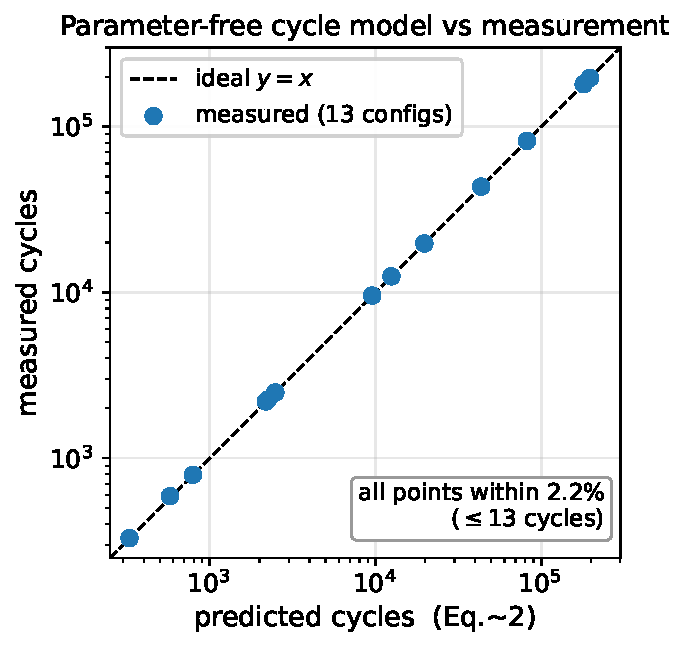
\includegraphics[width=\columnwidth]{fig5_cycle_model.pdf}
\caption{Validation of the parameter-free cycle model~\eqref{eq:cyc}: measured
vs.\ predicted cycles for all 13 configurations (dashed line is $y=x$). Every
point lies within $2.2\%$ ($\le$13 cycles) of the model.}
\label{fig:cyc}
\end{figure}

%% ===========================================================================
\section{Results}\label{sec:results}
%% ===========================================================================

\subsection{The full design grid}
Table~\ref{tab:grid} lists every Fermat-valid $(L,d)$ configuration with its
routed resource usage, clock rate, cycle count, and latency. All but the two
oldest designs close timing at $222$\,MHz (the $4.5$\,ns target); the $L=32$,
$d=2$ point closes at $180$\,MHz owing to a legacy twiddle convention and the
$L=32$, $d=3$ point at $236$\,MHz after retiming.

\begin{table*}[t]
\centering
\caption{Routed results for all 13 Fermat-valid configurations (U280, $4.5$\,ns
target). DSP equals the lane width $L$ in every case.}
\label{tab:grid}
\footnotesize
\setlength{\tabcolsep}{6pt}
\begin{tabular}{rrrrrrrrr}
\toprule
$L$ & $d$ & $N$ & LUT & FF & DSP & BRAM & $F_{\max}$ & Cycles\\
\midrule
8  & 2 & \num{64}    & \num{5698}  & \num{1548} & 8  & 0  & 222 & \num{329}\\
16 & 2 & \num{256}   & \num{14477} & \num{2949} & 16 & 0  & 222 & \num{793}\\
32 & 2 & \num{1024}  & \num{36839} & \num{5816} & 32 & 0  & 180 & \num{2489}\\
4  & 3 & \num{64}    & \num{2116}  & \num{908}  & 4  & 7  & 222 & \num{589}\\
8  & 3 & \num{512}   & \num{5452}  & \num{1616} & 8  & 14 & 222 & \num{2253}\\
16 & 3 & \num{4096}  & \num{13320} & \num{3026} & 16 & 28 & 222 & \num{12493}\\
32 & 3 & \num{32768} & \num{36539} & \num{5929} & 32 & 56 & 236 & \num{82112}\\
4  & 4 & \num{256}   & \num{2158}  & \num{924}  & 4  & 7  & 222 & \num{2197}\\
8  & 4 & \num{4096}  & \num{5624}  & \num{1641} & 8  & 14 & 222 & \num{19733}\\
4  & 5 & \num{1024}  & \num{2305}  & \num{940}  & 4  & 7  & 222 & \num{9565}\\
8  & 5 & \num{32768} & \num{6171}  & \num{1678} & 8  & 50 & 222 & \num{180573}\\
4  & 6 & \num{4096}  & \num{2360}  & \num{965}  & 4  & 7  & 222 & \num{43429}\\
4  & 7 & \num{16384} & \num{2543}  & \num{981}  & 4  & 25 & 222 & \num{197101}\\
\bottomrule
\end{tabular}
\end{table*}

\subsection{Fixed-width compute scaling in decomposition depth}
The clearest evidence is the $L=4$ column, isolated in Table~\ref{tab:l4} and
plotted in Fig.~\ref{fig:consthw}. From $d=3$ to $d=7$ the problem size grows by
$256\times$ (from $64$ to $16384$), yet the LUT count rises only from $2116$ to
$2543$ ($+20\%$) and the DSP count is fixed at $4$. The compute fabric is, to
first order, independent of $N$; memory and latency grow with $N$.

We are deliberately careful about the block-RAM column, which stays at $7$ tiles
for $N=64\ldots4096$ before stepping to $25$ at $N=16384$. The bank \emph{count}
is fixed at $L$ per memory ($3L=12$ data banks total); what changes is the number
of physical RAM tiles each bank occupies. The plateau is the FPGA allocation
quantum: each bank stores $N/L$ words of $17$ bits, so for $d\le 6$ a bank holds
at most $1024\times17\approx17.4$\,Kbit and fits in a single $18$-Kbit RAMB18
(half a $36$-Kbit tile); twelve half-tiles plus the twiddle ROM give the flat
$\approx7$ tiles, and the actual data ($3N\cdot17$, only $3.3$\,Kbit at $N=64$)
sits far below this floor. The step at $d=7$ is a tile-capacity crossing, not an
anomaly: the per-bank depth quadruples to $4096\times17\approx68$\,Kbit, which
exceeds one $36$-Kbit RAMB36 and forces \emph{two} tiles per bank
($12\times2+1\approx25$). Equivalently, $N$ has finally grown past the knee where
the $\Theta(N)$ data term overtakes the fixed floor: the $4\times$ increase in
$N$ ($4096\to16384$) yields $\approx3.6\times$ the BRAM ($7\to25$), tracking the
$\Theta(N)$ memory row of Table~\ref{tab:asymp}. A memory-bit efficiency
$\eta_{\mathrm{mem}}=\tfrac{3N\cdot17}{\text{allocated BRAM bits}}$ is below
$1\%$ at $N=64$ (floor-dominated) and only approaches useful utilization once
past the knee. We therefore claim fixed-width \emph{compute}, not constant
memory.

\begin{table}[t]
\centering
\caption{Fixed-width compute scaling at $L=4$. A $256\times$ increase in $N$
costs $+20\%$ LUTs and $0$ additional DSPs; BRAM is floor-dominated (flat at $7$
tiles) until $d=7$, where the per-bank depth exceeds one RAM tile and the
$\Theta(N)$ data term takes over.}
\label{tab:l4}
\footnotesize
\begin{tabular}{rrrrrr}
\toprule
$d$ & $N$ & LUT & DSP & BRAM & Latency\\
\midrule
3 & \num{64}    & \num{2116} & 4 & 7  & 2.65\,$\mu$s\\
4 & \num{256}   & \num{2158} & 4 & 7  & 9.89\,$\mu$s\\
5 & \num{1024}  & \num{2305} & 4 & 7  & 43.0\,$\mu$s\\
6 & \num{4096}  & \num{2360} & 4 & 7  & 195.4\,$\mu$s\\
7 & \num{16384} & \num{2543} & 4 & 25 & 887.0\,$\mu$s\\
\bottomrule
\end{tabular}
\end{table}

\begin{figure}[t]
\centering
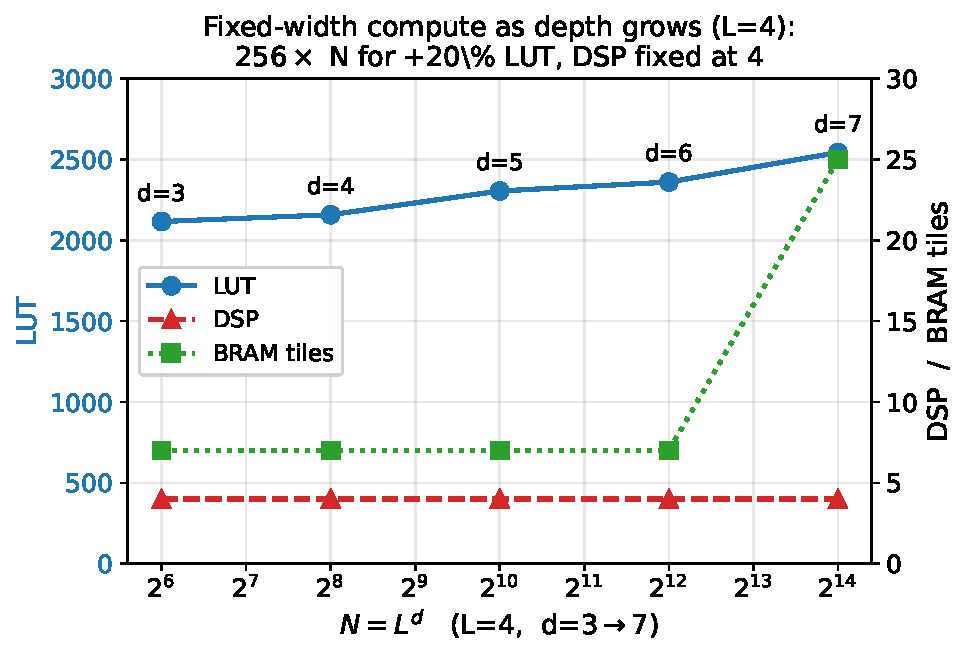
\includegraphics[width=\columnwidth]{fig2_constant_hw_L4.pdf}
\caption{Resource usage versus $N$ at $L=4$ ($d=3\ldots7$). LUT and DSP are
essentially flat; block-RAM is floor-dominated until the per-bank depth crosses
one RAM tile at $d=7$, after which it tracks the $\Theta(N)$ data.}
\label{fig:consthw}
\end{figure}

\subsection{Cost versus lane width}
The orthogonal sweep --- fixing $d=3$ and varying $L$ (Table~\ref{tab:lsweep})
--- shows the expected trade. DSP count scales exactly as $L$ (one modular
multiplier per lane), LUT scales sub-linearly (empirically $\approx L^{1.4}$),
and the per-coefficient cycle cost falls as $\approx 16/L+2.5$, so wider lanes buy
throughput at a super-linear logic cost.

\begin{table}[t]
\centering
\caption{Lane-width sweep at fixed depth $d=3$.}
\label{tab:lsweep}
\footnotesize
\begin{tabular}{rrrrrr}
\toprule
$L$ & $N$ & LUT & DSP & Latency & cyc/coef\\
\midrule
4  & \num{64}    & \num{2116}  & 4  & 2.65\,$\mu$s & 9.20\\
8  & \num{512}   & \num{5452}  & 8  & 10.1\,$\mu$s & 4.40\\
16 & \num{4096}  & \num{13320} & 16 & 56.2\,$\mu$s & 3.05\\
32 & \num{32768} & \num{36539} & 32 & 347\,$\mu$s  & 2.51\\
\bottomrule
\end{tabular}
\end{table}

\subsection{Shift-only versus DSP-based sub-NTT}
To quantify the value of the multiplier-free kernel we compare, at an identical
operating point ($N=4096$, $d=4$, $L=8$), our shift-only bidirectional sub-NTT
against a baseline that implements the same $8$-point transform with DSP-based
modular multipliers (Fig.~\ref{fig:kernel}). The shift-only kernel reduces LUTs by
$49\%$ ($5624$ vs $11040$), DSPs by $78\%$ ($8$ vs $37$), and improves $F_{\max}$
by $3.6\times$ ($222$ vs $61$\,MHz). We note for fairness that the baseline is a
\emph{representative, lightly-pipelined} DSP DFT rather than an aggressively
optimized one; its low $F_{\max}$ reflects an unbroken multiply--accumulate
critical path, and a deeper-pipelined DSP kernel would narrow the clock gap at
the cost of more registers. The point of the comparison is not the precise
ratio but the qualitative result: exploiting the power-of-two Fermat roots
removes the butterfly multipliers entirely, which is the correct kernel choice at
every lane width admissible under the modulus.

\begin{figure}[t]
\centering
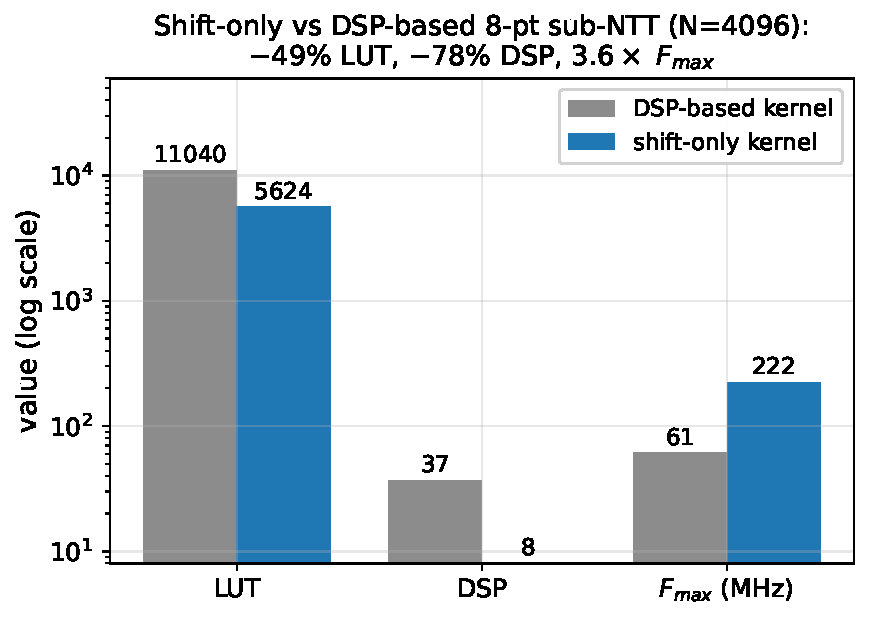
\includegraphics[width=\columnwidth]{fig3_shiftonly_vs_dsp.pdf}
\caption{Shift-only versus DSP-based $8$-point sub-NTT at $N=4096$, $d=4$:
$-49\%$ LUT, $-78\%$ DSP, $3.6\times$ $F_{\max}$ (log scale).}
\label{fig:kernel}
\end{figure}

\subsection{Power and energy}
A natural worry about a ``fixed-width'' claim is that constant logic might hide
growing switching activity. Table~\ref{tab:power} reports Vivado vectorless
power estimates for the routed designs (the absolute values are device-static
dominated --- the U280 contributes $\approx3.1$\,W of static power independent of
the design --- so the architecturally meaningful quantity is the \emph{dynamic}
power). At $L=4$ the dynamic power is essentially flat, $0.18\pm0.01$\,W across
$d=3\ldots6$, rising only to $0.24$\,W at $d=7$ when the BRAM count grows; the
\emph{switching} of the compute fabric does not scale with depth, mirroring the
flat LUT/DSP curves. Dynamic power instead tracks the lane width: the $L=8$
designs draw $0.32$--$0.42$\,W, $\approx2\times$ the $L=4$ value, consistent with
twice the lanes. Energy per multiplication grows with latency (a single product
of a larger polynomial does more total work), but energy \emph{per coefficient}
is roughly constant within a lane width ($0.13$--$0.18$\,nJ at $L=4$) and lower
at $L=8$ ($\approx0.08$\,nJ), since wider lanes amortize the per-cycle overhead.
These are vectorless estimates with default activity; an activity-annotated
(SAIF) study is future work.

\begin{table}[t]
\centering
\caption{Vivado vectorless power/energy (U280). Total power is device-static
dominated ($\approx3.1$\,W); dynamic power is the architecturally relevant figure
and stays flat with depth at fixed $L$.}
\label{tab:power}
\footnotesize
\setlength{\tabcolsep}{4pt}
\begin{tabular}{rrrrrr}
\toprule
$L$ & $d$ & $N$ & $P_{\mathrm{dyn}}$ (W) & $P_{\mathrm{tot}}$ (W) & $E$/coef (nJ)\\
\midrule
4 & 3 & \num{64}    & 0.181 & 3.31 & 0.14\\
4 & 4 & \num{256}   & 0.180 & 3.31 & 0.13\\
4 & 5 & \num{1024}  & 0.176 & 3.31 & 0.14\\
4 & 6 & \num{4096}  & 0.188 & 3.32 & 0.16\\
4 & 7 & \num{16384} & 0.243 & 3.38 & 0.18\\
8 & 4 & \num{4096}  & 0.317 & 3.45 & 0.075\\
8 & 5 & \num{32768} & 0.416 & 3.55 & 0.088\\
\bottomrule
\end{tabular}
\end{table}

%% ===========================================================================
\section{Comparison with prior work}\label{sec:compare}
%% ===========================================================================
The most directly comparable design is the recent iterative high-radix
Fermat-modulus NTT of Xing \emph{et al.}~\cite{xing2025}, which targets the same
modulus. Their published single-engine radix-16 point at $N=1024$ uses
$9783$ LUTs, $16$ DSPs, $0$ block-RAM, and reaches $2.6\,\mu$s at $274$\,MHz.
Table~\ref{tab:compare} places it beside our two $N=1024$ configurations and the
derived area--time products.

\begin{table}[t]
\centering
\caption{Head-to-head at the only overlapping size, $N=1024$. ATP is
area$\times$latency (lower is better).}
\label{tab:compare}
\footnotesize
\setlength{\tabcolsep}{3pt}
\begin{tabular}{lrrrrr}
\toprule
Design & LUT & DSP & Lat. & LUT-ATP & DSP-ATP\\
       &     &     & ($\mu$s) & (LUT$\cdot\mu$s) & (DSP$\cdot\mu$s)\\
\midrule
Ours, $L{=}32,d{=}2$ & \num{36839} & 32 & 13.8 & \num{509402} & 442\\
Ours, $L{=}4,d{=}5$  & \num{2305}  & 4  & 43.1 & \num{99312}  & 172\\
Xing \emph{et al.}~\cite{xing2025} & \num{9783} & 16 & \textbf{2.6} & \textbf{\num{25422}} & \textbf{41.6}\\
\bottomrule
\end{tabular}
\end{table}

We report this comparison without spin. At $N=1024$ the iterative design of
\cite{xing2025} is more efficient on \emph{every} area--time metric --- latency,
LUT-ATP, DSP-ATP, and throughput per unit area --- because a well-pipelined
iterative high-radix engine simply does more useful work per cycle than a
depth-multiplexed hierarchy at this small size. The hierarchical design's only
favorable axes are \emph{absolute} footprint (its smallest point uses $4$ DSPs
and $2.3$\,K LUTs, albeit at $\sim\!16\times$ the latency) and validated operation
across the full Fermat-valid range up to $N=32768$ at the same modulus, a regime
not reported by~\cite{xing2025}. The throughput-normalized view is equally
candid: at $N=1024$ \cite{xing2025} delivers $\approx394$\,Mcoef/s versus our
$24$--$74$\,Mcoef/s, and it leads on coefficients/s-per-DSP and per-kLUT as well.
Fig.~\ref{fig:atp} shows area--time product versus $N$ for the full grid with the
reference point overlaid.

\begin{figure}[t]
\centering
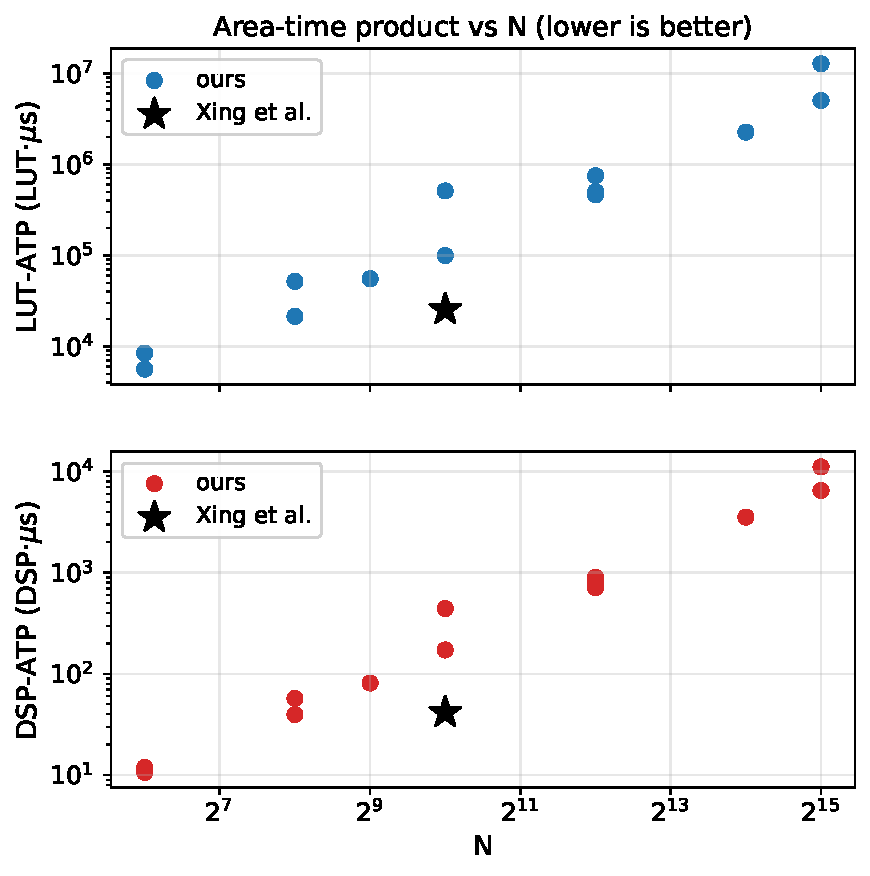
\includegraphics[width=\columnwidth]{fig4_atp_vs_n.pdf}
\caption{Area--time product versus $N$ for all configurations (top: LUT-ATP;
bottom: DSP-ATP), with the reference iterative design~\cite{xing2025} overlaid at
$N=1024$. The reference point sits below our cells on both metrics.}
\label{fig:atp}
\end{figure}

%% ===========================================================================
\section{Discussion and Limitations}\label{sec:disc}
%% ===========================================================================
The study is deliberately bounded by the modulus. Under $q=2^{16}+1$ the size is
capped at $N\le 32768$; the multi-megapoint regime that motivates streaming
multi-step NTTs is unreachable without a residue-number-system decomposition or a
larger Fermat prime, both left to future work. Within that bound, the experiments
make two facts concrete. First, hierarchical decomposition is \emph{not} the
efficient choice at small $N$, where a strong iterative design dominates; its
value lies in the scaling behavior and the minimal-footprint corner rather than
in raw efficiency. Second, the fixed-width compute behavior is real and measured,
and it is consistent with the transpose-free $O(L)$ interconnect: because neither
the interconnect nor the working-buffer count grows with $N$, the flat LUT/DSP
curves of Fig.~\ref{fig:consthw} are an expected outcome of the architecture
rather than a coincidence. Practical relevance is bounded: at $N\le 32768$ a
single engine targets lower-parameter lattice schemes, while in a
residue-number-system FHE pipeline it would act as one per-channel block ---
a multi-channel integration we leave to future work. The width-invariant regime
is also of interest beyond FPGA: on ASIC, a fixed-$L$ datapath with an $O(L)$
local interconnect and conflict-free SRAM banks would keep wirelength and
routing complexity bounded as $N$ grows --- the same property that keeps our
post-route $F_{\max}$ flat at $222$\,MHz across depth here. We characterize a
single device family and a single modulus; the dynamic power reported in
Table~\ref{tab:power} corroborates the fixed-width claim at the activity level,
and an activity-annotated (SAIF) energy--delay study and a second device family
are the natural next extensions.

%% ===========================================================================
\section{Conclusion}\label{sec:concl}
%% ===========================================================================
We presented a fully placed-and-routed design-space exploration of a multivariate
Fermat-modulus NTT for negacyclic polynomial multiplication, covering every
configuration admissible under the Fermat-prime constraint. The data establish
fixed-width compute scaling in decomposition depth --- a $256\times$ growth in
$N$ for a $20\%$ LUT increase and zero additional multipliers at $L=4$ --- and tie
it to a transpose-free conflict-free banking scheme with an $O(L)$ interconnect.
A candid comparison shows the approach is outpaced on area--time efficiency by a
state-of-the-art iterative design at small $N$, while offering the smallest
absolute footprint and validated operation across the full Fermat-valid size
range. The contribution is reproducible measurement and architectural insight
into where hierarchical Fermat-NTT decomposition does and does not pay off.

%% ===========================================================================
\begin{thebibliography}{99}
\bibitem{cooleytukey} J.~W. Cooley and J.~W. Tukey, ``An algorithm for the
machine calculation of complex Fourier series,'' \emph{Math. Comput.}, vol.~19,
pp.~297--301, 1965.

\bibitem{agarwalburrus} R.~C. Agarwal and C.~S. Burrus, ``Fast convolution using
Fermat number transforms with applications to digital filtering,'' \emph{IEEE
Trans. Acoust., Speech, Signal Process.}, vol.~22, no.~2, pp.~87--97, 1974.

\bibitem{bailey1990} D.~H. Bailey, ``FFTs in external or hierarchical memory,''
\emph{J. Supercomput.}, vol.~4, no.~1, pp.~23--35, 1990.

\bibitem{longa2016} P.~Longa and M.~Naehrig, ``Speeding up the number theoretic
transform for faster ideal lattice-based cryptography,'' in \emph{Proc. CANS},
2016, pp.~124--139.

\bibitem{kim2024fermat} J.~Kim, A.~C. Mert, \emph{et al.}, ``Exploring the
advantages and challenges of Fermat NTT in FHE acceleration,'' in \emph{Advances
in Cryptology --- CRYPTO}, 2024. IACR ePrint 2024/314.

\bibitem{xing2025} Y.~Xing, G.~Li, Z.~Ye, R.~W.~L. Luk, D.~Chen, H.~Yan, and
R.~C.~C. Cheung, ``High-radix/mixed-radix NTT multiplication
algorithm/architecture co-design over Fermat modulus,'' \emph{IEEE Trans.
Comput.}, 2025.

\bibitem{kocer2024} E.~Ko\c{c}er \emph{et al.}, ``IO-optimized design-time
configurable negacyclic seven-step NTT architecture for FHE applications,'' in
\emph{Proc. GLSVLSI}, 2025. IACR ePrint 2024/1889.

\bibitem{wanggao2023} W.~Wang and X.~Gao, ``A scalable multi-dimensional NTT
accelerator on FPGA,'' 2023.

\bibitem{supranational} Supranational, ``Nantucket: an FPGA NTT engine,''
ZPrize technical report, 2023.
\end{thebibliography}

\end{document}
